\documentclass{article}
\usepackage[utf8]{inputenc}
\usepackage{epigraph}
\usepackage{listings}
\usepackage[spanish]{babel}
\usepackage{color}
\usepackage{graphicx}
\usepackage{tikz}
%\usepackage[export]{adjustbox}
%\usepackage{fontspec}
\usepackage[letterpaper, total={7in, 10in}]{geometry}
%\setmainfont{Neo Euler} % IBM 3270, TERMINESS TTF
\title{\centerline{\textbf{ALGORITMOS: AYUDANTÍA 6}}}
\author{Ayudante: Yerko Ortiz}
\date{}
\definecolor{mygreen}{rgb}{0,0.6,0}
\definecolor{mygray}{rgb}{0.5,0.5,0.5}
\definecolor{mymauve}{rgb}{0.58,0,0.82}

\lstset{ %
  backgroundcolor=\color{white},   % choose the background color
  basicstyle=\footnotesize,        % size of fonts used for the code
  breaklines=true,                 % automatic line breaking only at whitespace
  captionpos=b,                    % sets the caption-position to bottom
  commentstyle=\color{mygreen},    % comment style
  escapeinside={\%*}{*)},          % if you want to add LaTeX within your code
  keywordstyle=\color{blue},       % keyword style
  stringstyle=\color{mymauve},     % string literal style
  showstringspaces=false
}
\begin{document}

\maketitle
\begin{flushleft}
\begin{minipage}{.3\textwidth}
\epigraph{\textit{"Good abstractions turn a nearly impossible task into two manageable
    ones. The first one is defining and implementing the abstraction. The second is
    using these abstractions to solve the problem at hand."}}{Andrew Tanenbaum, 
    Modern Operating Systems.}
\end{minipage}
%\begin{minipage}{.35\textwidth}
%    \hspace{1cm}
%\end{minipage}
%\begin{minipage}{.3\textwidth}
%    \begin{centering}
%    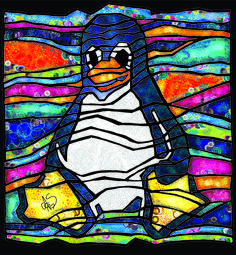
\includegraphics[scale=0.45]{CoolPenguin.jpg}
%    \end{centering}
%\end{minipage}
\newline
\textbf{Objetivo de la ayudantía: Resolver problemas de divide and
    conquer y un ejemplo de ordenamiento de strings}
\vspace{1cm}
\hrule
\vspace{1cm}
\section*{\centerline{Máximo prefijo en común}}
Dado un conjunto de N palabras, compute el máximo prefijo que tienen en común todas
las palabras del conjunto. El prefijo de un string se define como un substring de
caracteres adyacentes, donde el primer caracter del substring corresponde al primer
caracter del string. Por ejemplo sea la palabra banana, se dice que banan es
un prefijo de banana, así mismo ban es prefijo de banana, pero por otro lado anana no
es prefijo de banana.
\subsection*{Formato de la entrada}
\begin{itemize}
    \item La primera linea contiene un entero N que representa la cantidad de palabras.
    \item Las siguientes N lineas contienen N strings que representan la palabra $S_i$.
\end{itemize}
\subsection*{Dominio de la entrada}
\begin{itemize}
    \item $ 2 \leq N \leq 10^3$
    \item $ 1 \leq |S_i| \leq 100$
\end{itemize}
\subsection*{Formato de la salida}
\begin{itemize}
    \item Una linea que imprima el substring que corresponde al prefijo en común de
        largo máximo que las palabras tienen en común.
\end{itemize}
\subsection*{Caso de prueba}
\begin{itemize}
    \item \textbf{Entrada:} \newline
        5 \newline
        banana \newline barco \newline bardo \newline banal \newline baneado
    \item \textbf{Salida:} \newline
        ba
\end{itemize}
\vspace{0.5cm}
\hrule
\vspace{0.5cm}
\section*{\centerline{Diccionario de palabras}}
Franco tiene un sueño - el quiere crear su propio diccionario; esta no es una tarea fácil ya que el número de palabras que conoce, 
no es suficiente. Para compensar las pocas palabras que conoce piensa en una brillante idea: crear un diccionario usando
las palabras de algún libro en la biblioteca de su hermano. Su diccionario contendrá las palabras del libro ordenadas alfabeticamente
y sin palabras repetidas. 
\newline 
Su tarea como ninja de la programación es diseñar e implementar un programa en java, que simule el proceso que
Franco realiza para crear su diccionario.
\newline
\textbf{Nota:} su programa debe ser case insensitive(tomar todas las letras mayúsculas o minúsculas como si fuesen las mismas letras),
es decir que si por ejemplo su programa lee la palabra "naranja" la considera igual a la palabra "NaraNja".
\subsection*{Entrada}
\begin{itemize}
    \item La entrada consiste en un texto T con no más de 5000 lineas, cada linea tiene a lo más 200 caracteres. 
        El input termina con EOF.
\end{itemize}
\subsection*{Dominio}
\begin{itemize}
        \item $ 0 \leq |T| \leq 10 ^ 6$
\end{itemize}
\subsection*{Salida}
\begin {itemize}
    \item Las palabras del diccionario ordenadas de forma alfabética, 
        escritas en minúsculas y sin palabras repetidas.
\end {itemize}
\subsection*{Caso de prueba}
\begin{itemize}
    \item \textbf{Entrada:}\newline 
    Adventures in park.
    Two guys were going to the 
    park when they came to a fork in the
    road. The sign read: "park Closed." 
    So they went home.
    \item \textbf{Salida:} \newline
    \vspace{0.2 cm}
    \begin{minipage}[b]{.4\textwidth}
    \allowbreak
    \vspace{0.1cm}
    a \newline
    adventures \newline
    came \newline
    closed \newline
    fork \newline
    going \newline
    guys \newline
    home \newline
    in \newline
    park \newline
    read \newline
    \end{minipage}
    \begin{minipage}[b]{.4\textwidth}
    road \newline
    sign \newline
    so \newline
    the \newline
    they \newline
    to \newline
    two \newline
    went \newline
    were \newline
    when 
    \end{minipage}
\end{itemize}
\hrule 
\vspace{1cm}
\centerline{\textbf{Gracias por su atención!}}
\end{flushleft}
\end{document}


